\subsection{Improved correspondences}
We will now improve our precision of our correspondences by applying the Harris corner detector. This has been done by subtracting a small patch around our initial point location, and then run the Harris corner detector to find a more 'robust'/'easier to find again' location. These points have then been extracted and we can now estimate the fundamental matrix and scanline error to see if these improved points have an effect on the fundamental matrix estimation.

\subsubsection{Problems with Harris corner detection}
It is not obvious what the parameters for the Harris corner detector should be to give optimal results. Because a vast majority of the work in finding the improved points already was manual, I have tweaked the parameters for each original point until the Harris corner detector found a point which I would reckon would be easy to also find in the other image after applying the corner detector.

\subsubsection{Scanline agreement error}
If we simply estimate the fundamental with the improved correspondences we now find a \textbf{mean} of \textbf{1.92} and a \textbf{standard deviation} of \textbf{1.40} of the scanline agreement error. This is a fair bit better than running Ransac on the original correspondences. We can now run Ransac on the improved correspondences and see the result in \autoref{ImprovedRansac}.

\begin{figure}[h]
	\centering
	\begin{subfigure}{0.48\linewidth}
		\centering
		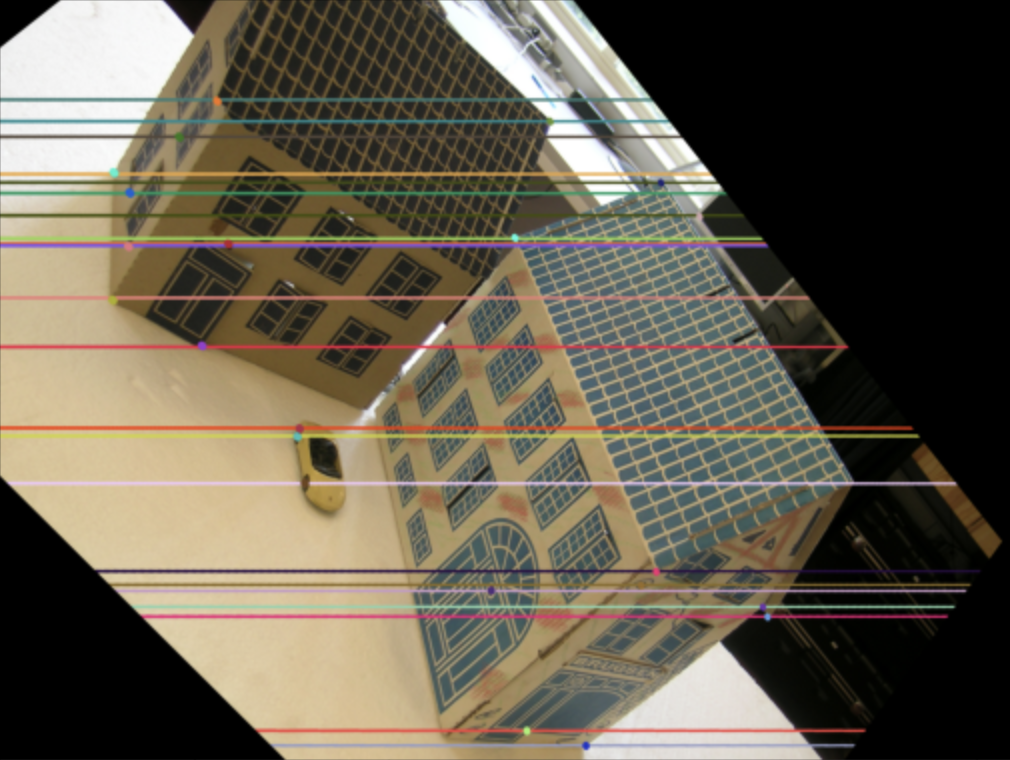
\includegraphics[width=\linewidth]{Materials/ImprovedARansac}
	\end{subfigure}
	\begin{subfigure}{0.48\linewidth}
		\centering
		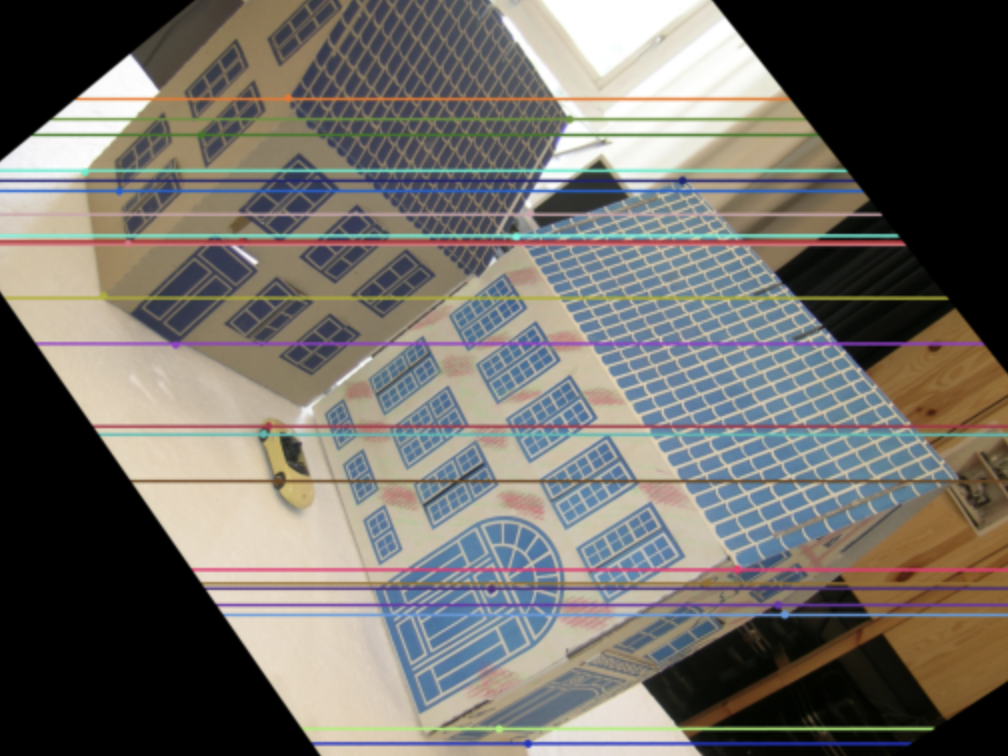
\includegraphics[width=\linewidth]{Materials/ImprovedBRansac}
	\end{subfigure}
	\caption{Result of using Ransac on the improved 25 correspondences before estimating the fundamental matrix and then bringing the images to scanline agreement.}
	\label{ImprovedRansac}
\end{figure}
We here find a \textbf{mean} of \textbf{1.52} and a \textbf{standard deviation} of \textbf{1.40} of the scanline agreement error, which is a slight improvement.

\subsubsection{Error as function of falsely added correspondences }
Looking at the error as a function of falsely added correspondences, now using the improved correspondences we get the results seen in \autoref{ImprovedRansacMedian}.

\begin{figure}[h]
	\centering
	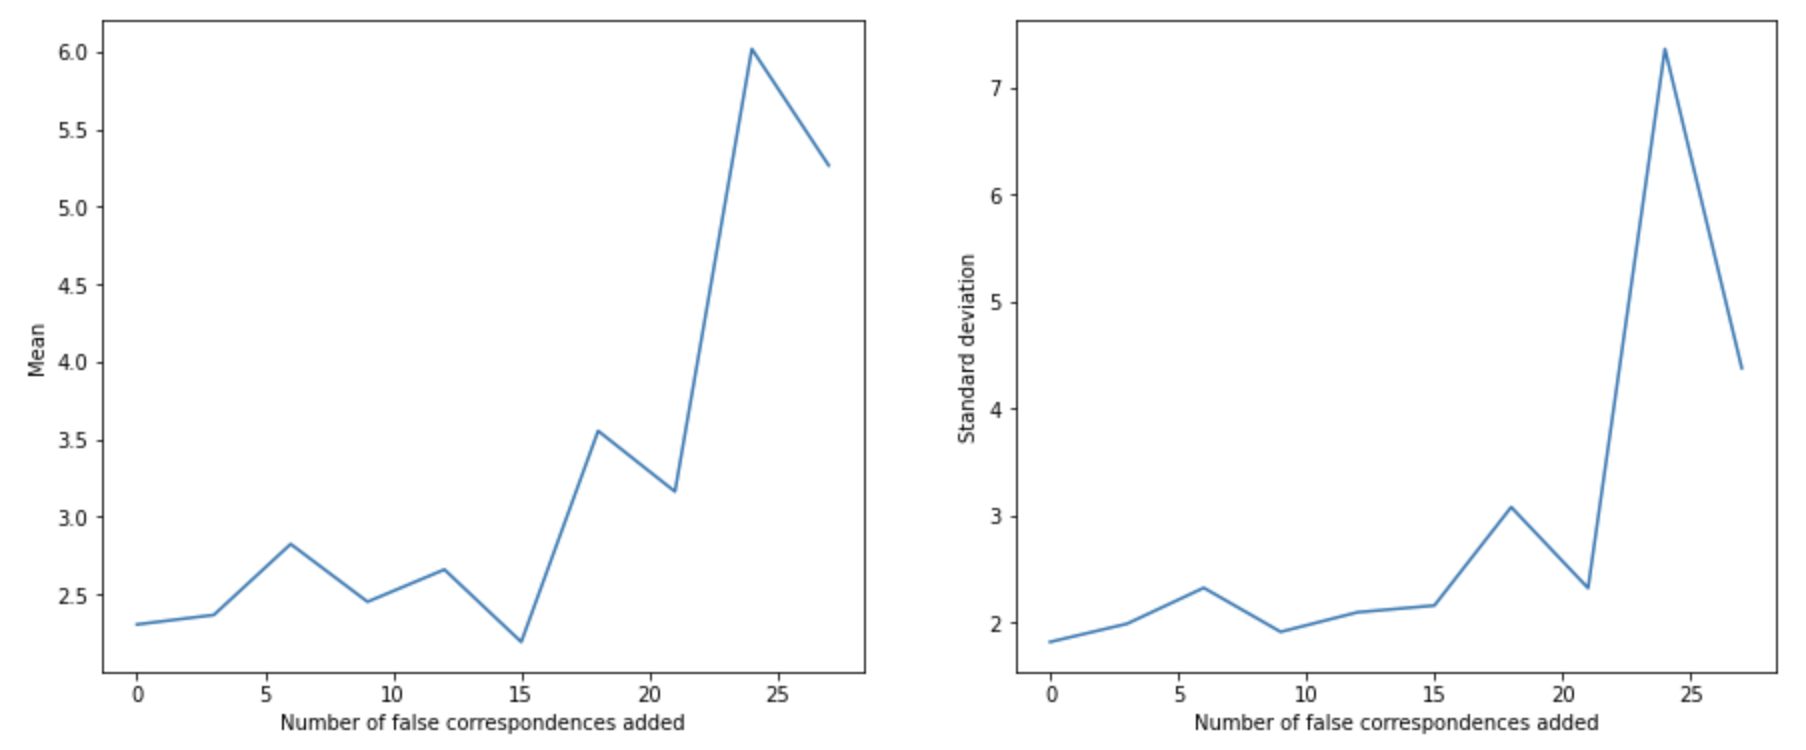
\includegraphics[width=\linewidth]{Materials/ImprovedRansacMedian}
	\caption{The median mean and standard deviation after 10 Ransac runs with increasing number of false correspondences added to the improved correspondences.}
	\label{ImprovedRansacMedian}
\end{figure}
We here see similar results as with the original correspondences, except a more clear tendency of increased error with increased number of false correspondences added. The more clear tendency might be a coincidence based on more similar Ransac runs or due to the run with 24 added false correspondences having a high error, and making it harder to see the small differences in mean and standard deviation. 